\subsection{Построение роутинга API}
Перед тем, как рассказывать о роутинге, необходимо пару слов сказать о конструкции ссылки на сайте или любом интернет ресурсе.

На рисунке~\ref{url-struct} написана структура абсолютно любой ссылки в интернете.
Как видно из рисунка, ссылка состоит из нескольких частей:
\begin{itemize}
    \item http-type,
    \item domain,
    \item route.
\end{itemize}

\begin{figure}
    \begin{lstlisting}[language=go]
    <http_type>://<domain>/<route>
    \end{lstlisting}
    \caption{Структура ссылки в интернете}
    \label{url-struct}
\end{figure}

Http-type --- это тип передачи HTTP пакета. Их есть 2 штуки:
\begin{itemize}
    \item http,
    \item https.
\end{itemize}

Обычная HTTP передача данный предполагает в себе открытую передачу данных. 
То есть абсолютно любой человек, который сможет поймать трафик, сможет увидеть все, что вы присылаете.
Очевидно, с таким способом передачи информации очень много проблем с безопасностью.

HTTPS --- это тот же HTTP, но S означает здесь secure.
Как понятно из определения, это означает, что при https передача HTTP пакета каким-то образом шифруется.
Для того, чтобы зашифровать данные, необходимо где-то найти сертификат и его переодически обновлять.
С помощью этого сертификата и шифруются данные.
Есть множество платных сетрификтов. Они чаще всего используются компаниями.
Однако, для обычного использования подойдет и бесплатный.
Современные браузеры научились предупреждать о любом http соединении, как о небезопасном и чаще всего могут запрещать их посещение.

Domain --- это домен. То есть по сути IP адрес сервера, на котором хостится сайт или API. 
Домен обычно в интернете скрыт под каким-то именем --- доменным.
Этот домен нужно воспринимать, как IP нашего сервера.

Итак, теперь мы подошли к части с route. 
Эту часть нужно воспринимать, как файловую систему компьютера.
Только за этим путем стоит какая-то функция, которая исполняется на фоне.
Сложность составления роутинга состоит в том, чтобы сделать эту файловую систему так, чтобы возможно было в ней ориентироваться и не потеряться.

Как в обычной файловой системе в директории мы можем увидеть только файлы или другие директории, так и тут мы не можем обращаться к промежуточным путям.
Для примера давайте посмотрим на рисунок~\ref{route-struct}.
Тут можно увидеть, что <<get\_address>> идет после api. Это значит, что по пути api мы не сможем повесить какой-либо хендлер.

\begin{figure}
    \begin{lstlisting}[language=go]
        \---api
        |   +---get_address
        |   +---set_address
    \end{lstlisting}
    \caption{Пример структуры роутинга}
    \label{route-struct}
\end{figure}

На рисунке приложения~\ref{route-struct-add} можно увидеть структуру роутинга api на момент написания ВКР.
Видно, что все хендлеры API расположены в одной структуре <<api>>. 
Все хендлеры, что относятся к взаимодействию с мангой расположены в директории <<manga>>. 
Хендлеры, отвечающие за регистрацию пользователей и прочую авторизацию расположены в директории <<login>>. 

<<Docs>> и <<docs-local>> созданы для того, чтобы можно было получить доступ к swagger.
На рисунке~\ref{swagger-pic} можно увидеть пример хендлеров, относящиеся к взаимодействию с мангой.

\begin{figure}
    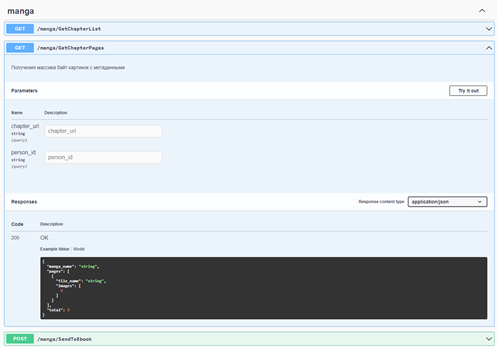
\includegraphics[scale=0.8]{imgs/swagger}
    \caption{SWAGGER представление хендлеров}
    \label{swagger-pic}
\end{figure}

\subsubsection{Описание хендлеров}
Основные хендлеры расположены в директории <<manga>>. 
Как можно увидеть из рисунка~\ref{route-struct} их на данным момент 4 штуки:
\begin{itemize}
    \item GetChapterList,
    \item GetChapterPages,
    \item GetChapterPagesPDF,
    \item SendToEbook.
\end{itemize}

Хендер <<GetChapterList>> отвечает за то, чтобы выдать структурировано информацию о доступных главах конкретной манги в виде ссылок.
Ссылки были выбраны потому, что с ними удобнее далее взаимодействовать на клиентских сервисах.

Хендлер <<GetChapterPages>> выдает картинки в отсортированной структуре. 
В структуре же находится байтовое представление картинки и вторым полем название файлы, чтобы удобнее потом было на клиентском сервисе собрать картинки вместе в нужном порядке.
Такое подход был выбран потому, что предполагается, что клиентские сервисы смогут самостоятельно отобразить картинки так, как это было бы удобнее всего для пользователя.

Хендлер <<GetChapterPagesPDF>> делает все то же самое, что и <<GetChapterPages>>, за исключением того, что в ответе получается файл pdf с уже собранной мангой.

Хендлер <<SendToEbook>> выполняет отправку сгенерированной манги на электронную книгу через электронную почту.
Обязательно присутствие электронной почты в базе данных.
